\section{Auswertung}
\label{sec:auswertung}

\cite{matplotlib} \cite{numpy}

\subsection{Magnetfeld}

\begin{figure}[H]
    \centering
    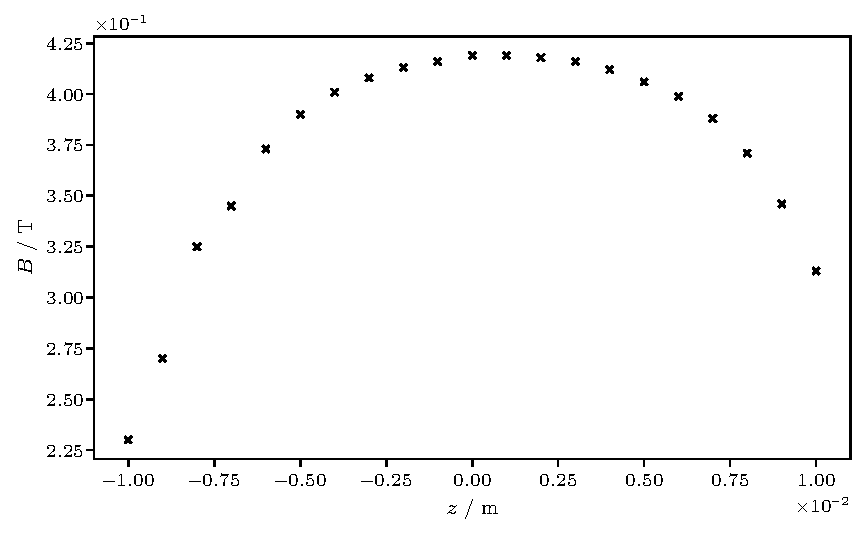
\includegraphics{build/field.pdf}
    \caption{Messung zum Verlauf des Magnetfeldes um den Luftspalt.}
    \label{fig:feld}
\end{figure}

\subsection{Faraday-Rotation}

\subsubsection{Dotierte Proben}

\begin{figure}[H]
    \centering
    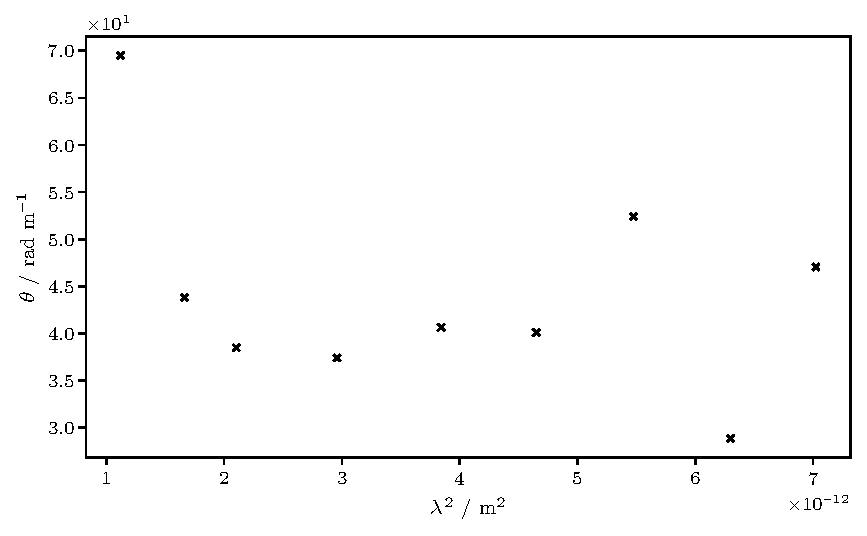
\includegraphics{build/doped-1.pdf}
    \caption{Messung zum normierten Drehwinkel für n-GaAs (1).}
    \label{fig:dotiert-1}
\end{figure}

\begin{figure}[H]
    \centering
    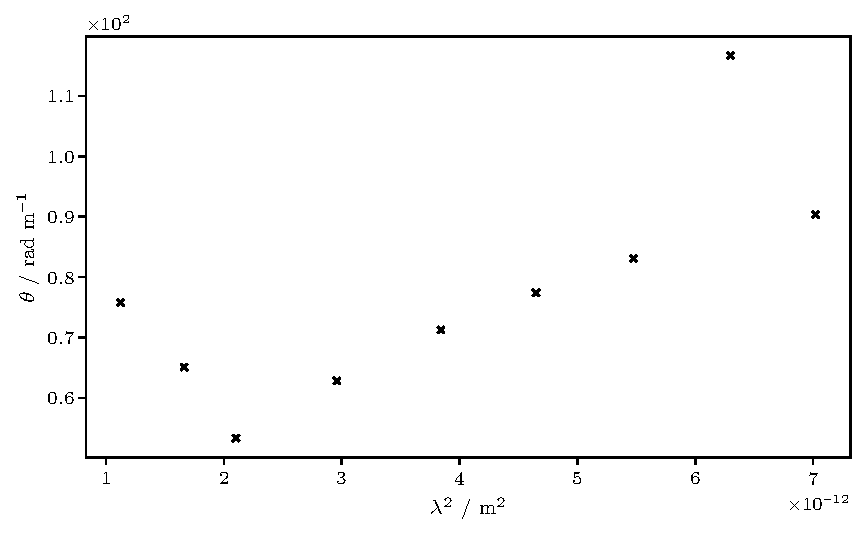
\includegraphics{build/doped-2.pdf}
    \caption{Messung zum normierten Drehwinkel für n-GaAs (2).}
    \label{fig:dotiert-2}
\end{figure}

\subsubsection{Reine Probe}

\begin{figure}[H]
    \centering
    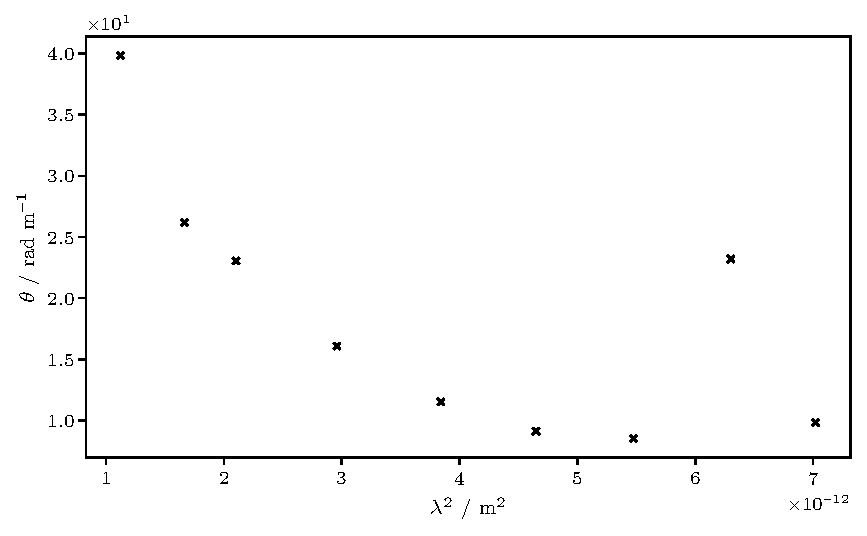
\includegraphics{build/pure.pdf}
    \caption{Messung zum normierten Drehwinkel für GaAs.}
    \label{fig:rein}
\end{figure}

\subsection{Effektive Masse}

$n = \num{3.4}$ \cite{brechungsindex} \eqref{eqn:ausgleichsrechnung}

\begin{align*}
    \pfrac{\theta}{L} = a \lambda^2 + b
\end{align*}

\begin{align*}
    m^* = \sqrt{\pfrac{Ne_0^3B}{8\pi^2 \varepsilon_0 c^3 n a}}
\end{align*}

\begin{align*}
    a = \input{build/a-1.tex} && b = \input{build/b-1.tex}
\end{align*}

\begin{align*}
    a = \input{build/a-2.tex} && b = \input{build/b-2.tex}
\end{align*}

\begin{figure}[H]
    \centering
    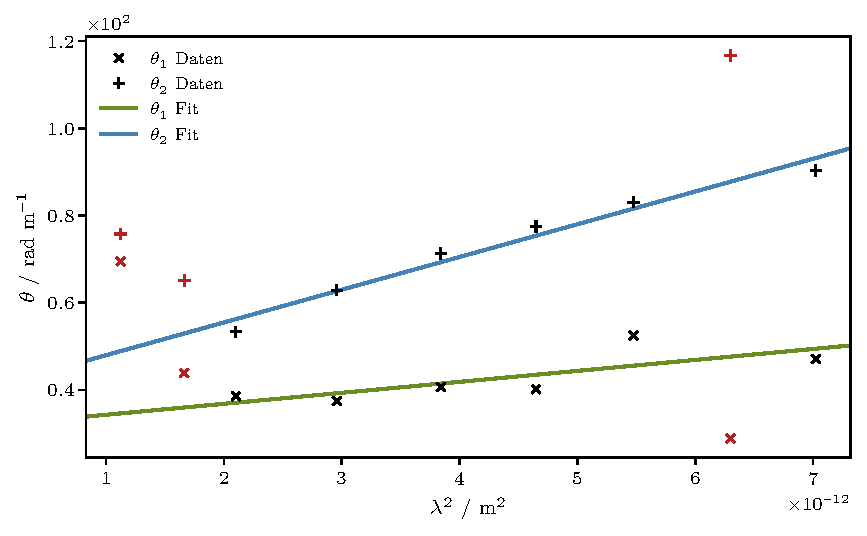
\includegraphics{build/mass.pdf}
    \caption{Ergebnisse und Ausgleichgeraden zum Drehwinkel aus Wirkung der Leitungselektronen.
             Hervorgehobene Datenpunkte werden ausgelassen.}
    \label{fig:masse}
\end{figure}
